\documentclass[11pt,table]{beamer}
\mode<presentation>
\usepackage{etex}
\usepackage{graphicx}
\usepackage{epstopdf}
\usepackage[english]{babel}
\usepackage{tabularx}
\usepackage{booktabs}
\usepackage{mathrsfs}
\usepackage{multicol}
\usepackage{bm}
\usepackage{subcaption}
\usepackage{wrapfig}
\usepackage{dcolumn}
\usepackage{threeparttable}
\usepackage{booktabs}
\usepackage{bbm}
\usepackage{amsmath,dsfont,listings}
\usepackage{amssymb}
\usepackage{rotating}
\usepackage{multirow}
\usepackage{tcolorbox}
\usepackage[authoryear]{natbib}
\usepackage{circledsteps}
\usepackage{qtree}

\usepackage{tikz}
\usetikzlibrary{arrows,decorations.pathmorphing,backgrounds,fit,positioning,shapes.symbols,chains}
\setbeamertemplate{section in toc}[sections numbered]
\setbeamertemplate{caption}[numbered]

\bibliographystyle{Econometrica}

\setbeamersize{text margin right=3.5mm, text margin left=7.5mm}  % text margin
\setbeamersize{sidebar width left=0cm, sidebar width right=0mm}
\setbeamertemplate{sidebar right}{}
\setbeamertemplate{sidebar left}{}

\definecolor{text-grey}{rgb}{0.45, 0.45, 0.45} % grey text on white background
\definecolor{bg-grey}{rgb}{0.66, 0.65, 0.60} % grey background (for white text)
\definecolor{fu-blue}{RGB}{0, 51, 102} % blue text
\definecolor{fu-green}{RGB}{153, 204, 0} % green text
\definecolor{fu-red}{RGB}{204, 0, 0} % red text (used by \alert)
\definecolor{BrewerBlue}{HTML}{377EB8} % Define Brewer Blue
\definecolor{BrewerRed}{HTML}{E41A1C}  % Define Brewer Red
\definecolor{BlueD}{HTML}{496a93}
\definecolor{BlueF}{HTML}{b9cde5}

\setbeamertemplate{frametitle}{%
    \vskip-30pt \color{text-grey}\large%
    \begin{minipage}[b][23pt]{\textwidth}%
    \flushleft\insertframetitle%
    \end{minipage}%
}

\setbeamertemplate{navigation symbols}{} 

%%% begin title page
\setbeamertemplate{title page}{
\vskip2pt\hfill
\vskip19pt\hskip3pt

% set the title and the author
\vskip4pt
\parbox[top][1.35cm][c]{11cm}{\LARGE\color{text-grey} \textcolor{red1}{RL}earning:\\[1ex] \inserttitle \\[1ex] \small \quad \\[3ex]}
\vskip17pt
\parbox[top][1.35cm][c]{11cm}{\small Unit 4-1: \insertsubtitle \\[2ex] \insertauthor \\[1ex]}
}
%%% end title page

%%% colors
\usecolortheme{lily}
\setbeamercolor*{normal text}{fg=black,bg=white}
\setbeamercolor*{alerted text}{fg=fu-red}
\setbeamercolor*{example text}{fg=fu-green}
\setbeamercolor*{structure}{fg=fu-blue}

\setbeamercolor*{block title}{fg=white,bg=black!50}
\setbeamercolor*{block title alerted}{fg=white,bg=black!50}
\setbeamercolor*{block title example}{fg=white,bg=black!50}

\setbeamercolor*{block body}{bg=black!10}
\setbeamercolor*{block body alerted}{bg=black!10}
\setbeamercolor*{block body example}{bg=black!10}

\setbeamercolor{bibliography entry author}{fg=fu-blue}
\setbeamercolor{bibliography entry journal}{fg=text-grey}
\setbeamercolor{item}{fg=fu-blue}
\setbeamercolor{navigation symbols}{fg=text-grey,bg=bg-grey}
%%% end colors

%%% headline
\setbeamertemplate{headline}{
\vskip30pt
}
%%% end headline

%%% footline
\newcommand{\footlinetext}{
%\insertshortinstitute, \insertshorttitle, \insertshortdate
}
\setbeamertemplate{footline}{
\vskip2pt
\hfill \raisebox{-1pt}{\usebeamertemplate***{navigation symbols}}
\hfill \insertframenumber\hspace{10pt}
\vskip4pt
}
%%% end footline

%%% settings for listings package
\lstset{extendedchars=true, showstringspaces=false, basicstyle=\footnotesize\sffamily, tabsize=2, breaklines=true, breakindent=10pt, frame=l, columns=fullflexible}
\lstset{language=Java} % this sets the syntax highlighting
\lstset{mathescape=true} % this switches on $...$ substitution in code
% enables UTF-8 in source code:
\lstset{literate={ä}{{\"a}}1 {ö}{{\"o}}1 {ü}{{\"u}}1 {Ä}{{\"A}}1 {Ö}{{\"O}}1 {Ü}{{\"U}}1 {ß}{\ss}1}
%%% end listings

\usepackage{concmath}
\usepackage{xcolor}
\definecolor{red1}{RGB}{206, 17, 38}
\definecolor{blue1}{RGB}{16, 118, 208}
\definecolor{gray1}{RGB}{117, 115, 115}
\usepackage{hyperref}


\newtheorem{proposition}{Proposition}
\newtheorem{assumption}{Definition}

\title[]{Short guides to reinforcement learning}
\subtitle[]{Neural Networks}
\author[D. Rostam-Afschar]{\textcolor{gray1}{Davud Rostam-Afschar (Uni Mannheim)}}
\date[]{\today}
\subject{Econometrics}
\renewcommand{\footlinetext}{\insertshortinstitute, \insertshorttitle, \insertshortdate}
\hypersetup{
    bookmarks=false,
    unicode=false,
    pdftoolbar=false,
    pdffitwindow=true,
    pdftitle={Reinforcement Learning for Business, Economics, and Social Sciences: \insertsubtitle},
    pdfauthor={Davud Rostam-Afschar},
    pdfsubject={Reinforcement Learning},
    pdfkeywords={reinforcement learning, Neural Networks},
    pdfnewwindow=true,
}
\def\sym#1{\ifmmode^{#1}\else\(^{#1}\)\fi}

\begin{document}

\begin{frame}[plain]
  \titlepage
\end{frame}

% --------------------------------------------------- Slide --
%\begin{frame}
	%\frametitle{Content}
	%\tableofcontents[]
%\end{frame}

\section{Neural Networks}
{
\setbeamercolor{background canvas}{bg=BrewerBlue}
\begin{frame}
\centering
\Huge
\textcolor{white}{How to deal with very large state-action spaces?}
\thispagestyle{empty}
\end{frame}
}



\begin{frame}{Tabular Value Iteration and Q-Learning}


  \begin{itemize}
      \item  Markov Decision Processes: value iteration 
      
      $$V(s) \leftarrow \max _{a} R(s)+\gamma \sum_{s^{\prime}} \mathbb{P}\left(s^{\prime} \mid s, a\right) V\left(s^{\prime}\right)$$

\item  Reinforcement Learning: Q-Learning

$$
Q(s, a) \leftarrow Q(s, a)+\alpha\left[r+\gamma \max _{a} Q\left(s^{\prime}, a^{\prime}\right)-Q(s, a)\right]
$$

\item  Complexity depends on number of states and actions 
  \end{itemize}  
\end{frame}

    \begin{frame}{Large State Spaces}

\begin{columns}[T]
\begin{column}{0.6\textwidth}
\begin{itemize}
    
 \item  Computer Go: $3^{361}$ states
 \end{itemize}
\end{column}
\begin{column}{0.4\textwidth}
\centering
\includegraphics[width=0.6\textwidth]{figures/go.png}
\end{column}
\end{columns}

\begin{columns}[T]
\begin{column}{0.6\textwidth}
\begin{itemize}
    \item Inverted pendulum: $\left(x, x^{\prime}, \theta, \theta^{\prime}\right)$
\begin{itemize}
     
 \item 4-dimensional

\item continuous state space 
\end{itemize}
\end{itemize}
\end{column}
\begin{column}{0.4\textwidth}
\vspace{5mm}
\centering
\scalebox{0.25}{
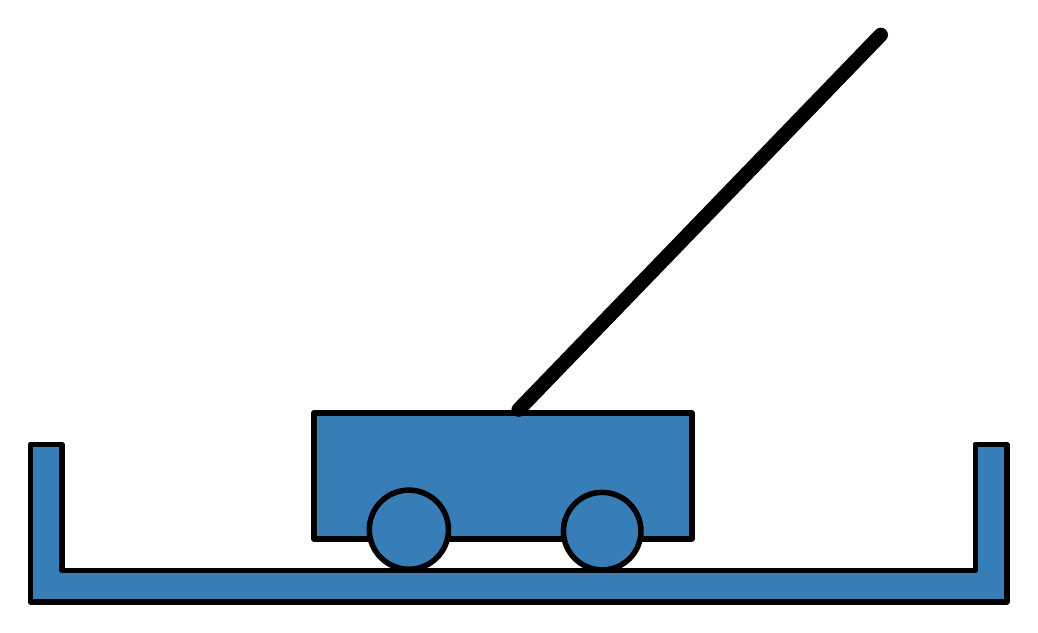
\begin{tikzpicture}[line cap=round,line join=round,scale=2]

\fill[draw=black,line width=1.5pt,line width=2pt,fill=BrewerBlue] (-6.4,-0.6) -- (-6.2,-0.6) -- (-6.2,-1.4) -- (-0.4,-1.4) -- (-0.4,-0.6) -- (-0.2,-0.6) -- (-0.2,-1.6) -- (-6.4,-1.6) -- cycle;
\fill[draw=black,line width=1.5pt,line width=2pt,fill=BrewerBlue] (-4.6,-0.4) -- (-2.2,-0.4) -- (-2.2,-1.2) -- (-4.6,-1.2) -- cycle;
\draw [line width=5.2pt] (-3.3,-0.38)-- (-1,2);
\draw [draw=black,line width=1.5pt,line width=2pt,fill=BrewerBlue] (-3.9967614229502813,-1.1421149589850645) circle (0.25130295023545973cm);
\draw [draw=black,line width=1.5pt,line width=2pt,fill=BrewerBlue] (-2.769226119268462,-1.151278199750565) circle (0.24609780622142172cm);


%\draw (-1.3,-1) node {\huge \textbf{Environment}};
%\draw (-1.5,2.8) node {\huge \textbf{Agent}};
%\draw (-6,1) node {\Large \textbf{State}};
%\draw (-2,1) node {\Large \textbf{Reward}};
%\draw (1.5,1) node {\Large \textbf{Action}};
\end{tikzpicture}
}

\end{column}
\end{columns}
\vspace{3mm}
\begin{itemize}
    \item Atari: $210 \times 160 \times 3$ dimensions (pixel values) 
\end{itemize}

\begin{center}
    \includegraphics[width=1\textwidth]{figures/atari games.png}
\end{center}
        
    \end{frame}
    
\begin{frame}{Functions to be Approximated}


   \begin{itemize}
       \item  Policy: $\pi(s) \rightarrow a$\\[2ex]

\item  Value function: $V(s) \in \mathbb{R}$\\[2ex] 

\item  Q-function: $Q(s, a) \in \mathbb{R}$

   \end{itemize} 
\end{frame}

\begin{frame}{Q-function Approximation}


    \begin{itemize}
        \item  Let $s=\left(x_{1}, x_{2}, \ldots, x_{n}\right)$\\$\rightarrow$ states are defined by a vector of features $x$.

\item  Linear

$$
Q(s, a) \approx \sum_{i} w_{a i} x_{i}
$$

\item  Non-linear (e.g., neural network)

$$
Q(s, a) \approx g(\boldsymbol{x} ; \boldsymbol{w})
$$ 
    \end{itemize}
\end{frame}




\section{Traditional Neural Network}

\begin{frame}{Traditional Neural Network}

\begin{columns}[T]
\begin{column}{0.4\textwidth}

\begin{itemize}
\item  Network of units  (computational neurons)  linked by weighted edges
\end{itemize}
\end{column}
\begin{column}{0.6\textwidth}
\centering
\includegraphics[width=0.8\textwidth]{figures/4.png}
\end{column}
\end{columns}

\begin{itemize}
    \item Each unit computes: 

    $z=h(\boldsymbol{w}'\boldsymbol{x}+b)$

    \begin{itemize}
        \item Inputs: $\boldsymbol{x}$
\item Output: $z$
\item Weights (parameters): $\boldsymbol{w}$
\item Bias: $b$
\item Activation function (usually non-linear): $h$
 
    \end{itemize}
\end{itemize}
\begin{footnotesize}
\textbf{Readings: Deep Neural Networks}
\citet[][chapters 6, 7, 8]{goodfellow2016deep}
\end{footnotesize}
\end{frame}


\begin{frame}{One hidden Layer Architecture}

\begin{itemize}
    \item Feed-forward neural network
 
\end{itemize}
    \begin{center}
\begin{tikzpicture}[x=100pt,y=50pt,
        N/.style={circle,draw=BlueD,fill=BlueF,line width=1pt,inner sep=0pt,align=center},
        BN/.style={N,text width=14pt},
        SN/.style={N,text width=10pt},
        E/.style={>=latex,line width=1pt},
        En/.style={font=\footnotesize,inner sep=1pt},
    ]
    %
    \node[BN] (x1) at (1,2) {$x_1$};
    \node[BN] (x2) at (1,1) {$x_2$};
    %
    \node[BN] (z1) at (2,2) {$z_1$};
    \node[BN] (z2) at (2,1) {$z_2$};
    %
    \node[BN] (y1) at (3,1.5) {$y_1$};
    %
    \node[SN] (s1) at (1.3,2.7) {$1$};
    \node[SN] (s2) at (2.3,2.7) {$1$};
    %
    \draw[E,->] (x1)--(z1) node[En,pos=0.3,above]{$w_{11}^{(1)}$};
    \draw[E,->] (x1)--(z2) node[En,pos=0.3,above right,inner sep=0pt]{$w_{21}^{(1)}$};
    %
    \draw[E,->] (x2)--(z1) node[En,pos=0.3,below right,inner sep=0pt]{$w_{12}^{(1)}$};
    \draw[E,->] (x2)--(z2) node[En,pos=0.3,below]{$w_{22}^{(1)}$};
    %
    \draw[E,->] (z1)--(y1) node[En,pos=0.5,above]{$w_{11}^{(2)}$};
    \draw[E,->] (z2)--(y1) node[En,pos=0.5,below]{$w_{12}^{(2)}$};
    %
    \draw[E,->] (s1)--(z1) node[En,pos=0.3,above right]{$b_{1}^{(1)}$};
    \draw[E,->] (s1)--(z2) node[En,pos=0.8,above right]{$b_{2}^{(1)}$};
    \draw[E,->] (s2)--(y1) node[En,pos=0.3,above right]{$b_{1}^{(2)}$};
    %
    %
    \node[above] at (x1.north) {\strut Input};
    \node[above] at (z1.north) {\strut Hidden};
    \node[above] at (y1.north) {\strut Output};
\end{tikzpicture}
    \end{center}

\begin{itemize}
    \item Hidden units: $z_{j}=h_{1}\left(\boldsymbol{w}_{j}^{'(1)} \boldsymbol{x} +b_{j}^{(1)}\right)$ 

    \item  Output units: $y_{k}=h_{2}\left(\boldsymbol{w}_{k}^{'(2)} \boldsymbol{z} +b_{k}^{(2)}\right)$

    \item  Overall: $y_{k}=h_{2}\left(\sum_{j} w_{k j}^{(2)} h_{1}\left(\sum_{i} w_{j i}^{(1)} x_{i}+b_{j}^{(1)}\right)+b_{k}^{(2)}\right)$
\end{itemize}
    
\end{frame}



\section{Common Activation Functions}
{
\setbeamercolor{background canvas}{bg=BrewerBlue}
\begin{frame}
\centering
\Huge
\textcolor{white}{Common Activation Functions}
\thispagestyle{empty}
\end{frame}
}

\begin{frame}{Common activation functions $h$}
    \begin{columns}[T]
\begin{column}{0.4\textwidth}
\begin{itemize}
    \item  Threshold: $h(a)=\left\{\begin{array}{cc}1 & a \geq 0 \\ -1 & a<0\end{array}\right.$\\[3ex]

\uncover<2->{    \item  Sigmoid: $h(a)=\sigma(a)=\frac{1}{1+e^{-a}}$
}
\end{itemize}
\end{column}
\begin{column}{0.6\textwidth}
\centering
\uncover<3>{\includegraphics[width=1\textwidth]{figures/6.png}
}
\end{column}
\end{columns}
\vspace{4mm}

\begin{columns}[T]
\begin{column}{0.4\textwidth}
\begin{itemize}
\uncover<4->{    \item  Gaussian: $h(a)=e^{-\frac{1}{2}\left(\frac{a-\mu}{\sigma}\right)^{2}}$\\[3ex]}
\uncover<5->{    \item  $\operatorname{Tanh}: h(a)=\tanh (a)=\frac{e^{a}-e^{-a}}{e^{a}+e^{-a}}$\\[3ex]}
\uncover<7->{    \item Identity: $h(a)=a$}
\end{itemize}
\end{column}
\begin{column}{0.6\textwidth}
\centering
\uncover<6>{\includegraphics[width=1\textwidth]{figures/7.png}}
\end{column}
\end{columns}

\end{frame}



\section{Universal Function Approximation}
{
\setbeamercolor{background canvas}{bg=BrewerBlue}
\begin{frame}
\centering
\Huge
\textcolor{white}{Universal Function Approximation}
\thispagestyle{empty}
\end{frame}
}


\begin{frame}{Universal function approximation}


\begin{itemize}
    \item \textbf{Theorem:} Neural networks with at least one hidden  layer of sufficiently many sigmoid/tanh/Gaussian  units can approximate any function arbitrarily closely.
 
\end{itemize}

\begin{center}
\includegraphics[width=0.9\textwidth]{figures/8.png}

\end{center}
    
\end{frame}

\begin{frame}{Minimize least squared error}


   \begin{itemize}
       \item  Minimize error function (Euclidian norm is commonly used for distance)

$$J(\boldsymbol{W})=\frac{1}{2} \sum_{n} J_{n}(\boldsymbol{W})^{2}=\frac{1}{2} \sum_{n}\left\|f\left(\boldsymbol{x}_{n}, \boldsymbol{W}\right)-y_{n}\right\|_{2}^{2}$$ 

where $J$ is the error function, $f$ is the function encoded by the neural net and $n$ is the number data points.

\item  Train by gradient descent (a.k.a. backpropagation)

\begin{itemize}
    \item  For each example $(\boldsymbol{x}_{n}, y_{n})$, adjust the weights as follows:

$$
w_{j i} \leftarrow w_{j i}-\alpha \frac{\partial J_{n}}{\partial w_{j i}}
$$ 
   \end{itemize} 
   \end{itemize}
	
	$\alpha$ is the stepsize.
\end{frame}

\begin{frame}{Minimize	least squared error}

\begin{itemize}
    \item Train by gradient descent (a.k.a. backpropagation)
\begin{itemize}
    \item For each example $(\boldsymbol{x}_{n}, y_{n})$, adjust the weights as follows:
 
\end{itemize} 
\end{itemize}

\begin{center}
   \includegraphics[width=0.85\textwidth]{figures/9.PNG} 
\end{center}
    
\end{frame}


\begin{frame}[t,allowframebreaks
]%\nocite{*}
\frametitle{References}
\small
\bibliography{bib}
\end{frame}
\section{Takeaways}
{
\setbeamercolor{background canvas}{bg=BrewerBlue}
\begin{frame}
\centering
\Huge
\textcolor{white}{Takeaways}
\thispagestyle{empty}
\end{frame}
}

\begin{frame}{Neural Nets to Approximate Policies, Value or Quality Functions}
\begin{itemize}
    \item Tabular methods fail in large or continuous state-action spaces\\[2ex]
    \item Neural networks approximate
		
		\begin{itemize}
			\item policies, 
			\item value functions, and
			\item Q-functions\\[2ex]
		\end{itemize}
		
    \item A basic network has 
		
		\begin{itemize}
			\item weighted inputs,
			\item nonlinear activations, and
			\item outputs\\[2ex]
		\end{itemize}
		
    \item Neural networks can approximate any continuous function (universal approximation)
\end{itemize}
\end{frame}


\end{document}
